\documentclass{article}
\usepackage[utf8]{inputenc}
\usepackage{amsmath}
\usepackage{amsthm}
\usepackage{graphicx}
\usepackage{geometry}
\usepackage{caption}
\usepackage{hyperref}
\usepackage{minted}
\usemintedstyle{manni}
\geometry{a4paper, portrait, margin=1in}

\theoremstyle{plain}
\newtheorem{thm}{Theorem}

\theoremstyle{definition}
\newtheorem{defn}{Definition} % definition numbers are dependent on theorem numbers
\newtheorem{exmp}{Example} % same for example numbers

\hypersetup{
    colorlinks=true,
    urlcolor=blue,
}

\title{Operating Systems (UE18CS302)\\
    \large Unit 5}
\author{Aronya Baksy}

\begin{document}
    \maketitle

\section{I/O Management}
\begin{itemize}
    \item The I/O subsystem is the part of the kernel that handles control of various types and generations of I/O devices and their interaction with the rest of the system.
    
    \item A device driver is a software abstraction layer between the OS and the actual hardware. It allows the OS to access the I/O device functionalities in an uniform manner irrespective of the physical nature of the device. 
    
    \item Conflicting trends in I/O device design are increased standardization of h/w and s/w interfaces, and an increasing variety of new I/O devices. 
\end{itemize}

\subsection{I/O Hardware}
\begin{itemize}
    \item A \textbf{port} is a physical interface via which the I/O device and the rest of the system communicate. 
    
    \item A \textbf{bus} is a set of wires and a protocol that defines the message formats that are exchanged on those wires. 
    
    \item \textbf{PCI buses} are used to connect the CPU-memory subsystem to fast I/O devices (like SSDs, graphics cards/GPUS and WiFi cards). \textbf{Expansion buses} are used to connect slower devices like keyboards and serial/USB ports. \textbf{SCSI buses} are used to connect printers or disks to computer systems. 
\end{itemize}

\begin{figure}[!h]
    \centering
    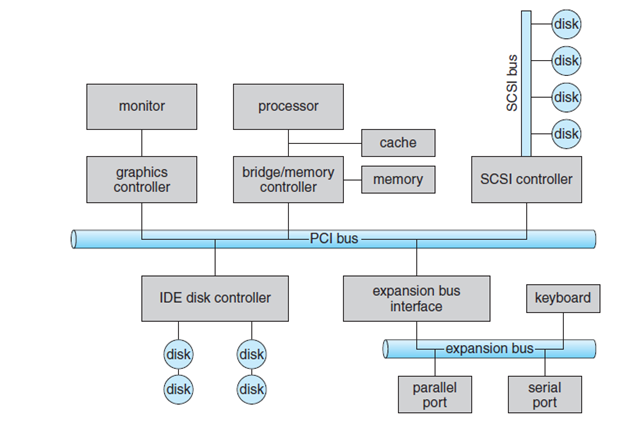
\includegraphics[scale=0.6]{os1.png}
    \caption{A typical bus layout}
    \label{fig:my_label_1}
\end{figure}

\begin{itemize}
    \item Other common bus technologies are \textbf{PCIe} (e for Express) that offers upto 16 GBps throughput and \textbf{HyperTransport} that offers upto 25 GBps throughput. 
    
    \item An \textbf{I/O Controller} is a collection of electronics that operate a port/device/bus. 
    \item Some bus architectures like serial have a simple controller (single chip that can control the signals on the bus). 
    
    \item More complex architectures like SCSI contain their own entire circuit boards that consist of processor, microcode instructions and some memory to process protocol messages. These circuti boards, also known as host adaptors, plug directly into the computer.
    
    \item Some devices have their own controllers (eg: disks, that implement the device side of SCSI or SATA protocol). 
\end{itemize}

\subsection{Communication between CPU and I/O Devices}
\begin{itemize}
    \item The CPU communicates with the I/O devices by writing control information to the registers that are present on the controller for that device. 
    
    \item This is done by the CPU using special I/O instructions that trigger flow of bytes or words into or out of a particular port address. 
    
    \item Alternately, memory mapped I/O is a feature that allows the CPU to view the device registers as an extension of the addressable memory space. The CPU writes/reads these registers using standard instructions at their mapped locations in physical memory. 
    
    \item Some devices use both. For example, graphics controllers have ports as well as a large set of registers to hold the screen contents. The CPU can change the screen contents by writing to these registers (faster than issuing many instructions to each port). 
    
    \item Memory mapped I/O can be overwritten by random processes that point to that memory by mistake. This can be solved using protected memory.
    
    \item The registers present on each I/O port are:
    \begin{enumerate}
        \item \textbf{Status Register}: Current status info of the I/O device that is read by the host (eg: current command completed, data available to read, device error occurred)
        
        \item \textbf{Control Register}: Written by the host to issue commands to the I/O device, or change its mode (eg: half/full duplex mode, enable error checking using parity bits, set word size, set speed of transfer).
        
        \item \textbf{Data-in Registers}: Read by the host to get input
        
        \item \textbf{Data-out Registers}: Written by the host to get output
    \end{enumerate}
\end{itemize}

\section{Polling}
\begin{itemize}
    \item Polling is a method used by host to perform I/O on a device. 
    
    \item The \textbf{busy} bit in the status register indicates the current status of the I/O device (busy or idle) 
    
    \item The \textbf{command-ready} bit in the control register indicates that the host is ready to send a command to the device controller. 
    
    \item The following steps take place in polling
    \begin{enumerate}
        \item The host reads the busy bit repeatedly until it is clear (0). 
        
        \item The host sets the write bit in the command register, and writes the byte of data into the data-out register. 
        
        \item The host then sets the command-ready bit in the control register. The controller notices this and sets the busy bit to 1. 
        
        \item The controller performs the I/O by seeing the write command from the control register and the data to be written from the data-out register. 
        
        \item Once the I/O is complete the command-ready bit is cleared, the error bit in the status register is cleared, and the busy bit is once again reset to 0. 
    \end{enumerate}
    
    \item This loop is repeated for each byte of data to be written. 
    
    \item In case there are long wait times for the device to be not busy, then the host might switch to another task, which leaves no mechanism for it to know when the device is free. 
    
    \item The process of servicing the device must be fast, or else data might be lost (eg: data coming in via keyboard might overflow the buffer if it is not written to the device fast enough). 
    
    \item The basic polling operations (read register, logical and for extracting a status bit, and branch if not zero) are fast instructions, but become inefficient when done repeatedly for no immediate reward. 
\end{itemize}

\section{Interrupts}
\begin{itemize}
    \item An interrupt is a mechanism by which an I/O device requests service from the host, rather than the host polling the device repeatedly. 
    
    \item The \textit{interrupt request line} is the method by which devices notify the CPU. As soon as a device \textit{raises} an interrupt on the request line, the CPU saves the current state, \textit{catches} the interrupt and \textit{dispatches} it to the interrupt handler routine (ISR). 
    
    \item The ISR determines the cause of the interrupt, handles it, and executes a return-from-interrupt instruction that restores the state of the CPU. This is called\textit{ clearing} the interrupt.  
    
    \item Additional features of Interrupt handling that are needed are:
    \begin{enumerate}
        \item Defer interrupt handling during critical processes
        
        \item Multilevel interrupts to separate high and low priority interrupts
        
        \item An efficient method of determining which device raised the interrupt (not polling)
    \end{enumerate}  
    
    \item Maskable interrupts can be turned off by the CPU while it performs some critical operations. Non-maskable interrupts cannot be turned off, and they normally indicate unrecoverable memory errors. 
    
    \item Interrupt hardware accepts an address which is an offset in the \textbf{interrupt vector table} that contains addresses of interrupt handlers for specific types. 
    
    \item In case of large number of devices and the associated large number of ISRs, \textbf{chained interrupts} allow the IVT to index to a linked list of interrupts. Each time an entry in the IVT is referenced, all the list entries are checked until one ISR is found in that list which can service the current interrupt. 
    
    \item An \textbf{exception} is an anomalous condition that requires special handling. Interrupts are used to handle specific exceptions.
    
    \item A \textbf{trap} or a \textbf{software interrupt} is an interrupt that is generated by a program running in user mode. It is used when an user program requests for service from the kernel via a system call. 
    
    \item Upon receipt of a trap instruction, the interrupt hardware saves the state of the user code, switches to kernel mode, and then dispatches to the kernel routine that implements that desired service. 
    
    \item Multithreaded kernels are useful for handling multiple interrupt priorities. (eg: In Solaris, interrupt handlers are implemented as kernel threads. Interrupt handling threads are issued high priorities, higher than application (user) threads, and they can preempt one another. 
\end{itemize}

\section{Dynamic Memory Access Controller (DMA)}
\begin{itemize}
    \item The DMA is a special-purpose controller that bypasses the CPU and manages I/O devices. It contains command register that is written to by the CPU. 
    
    \item DMA and device controllers perform a handshaking procedure across the \textbf{DMA-request} and \textbf{DMA-acknowledge} wires. The device controller places a signal on the request wire while it is interacting with the DMA, and removes that signal once the transfer is complete. 
    
    \item While the DMA uses the memory bus, the CPU cannot access main memory. This is referred to as \textbf{cycle stealing} where CPU execution cycles are being used by the DMA. Despite this phenomenon, DMA allows for better performance compared to non-DMA access. 
    
    \item There is a tradeoff between protected and non-protected kernels whether to give direct access of memory devices to user programs (ie. allow user programs to directly issue device commands, instead of using privileged system calls to do the same). 
    
    \item The tradeoff is between performance (the direct approach removes the overhead of kernel communication and context switching) and security (invalid access by user process can cause device errors or system crash). 
\end{itemize}

\begin{figure}[!h]
    \centering
    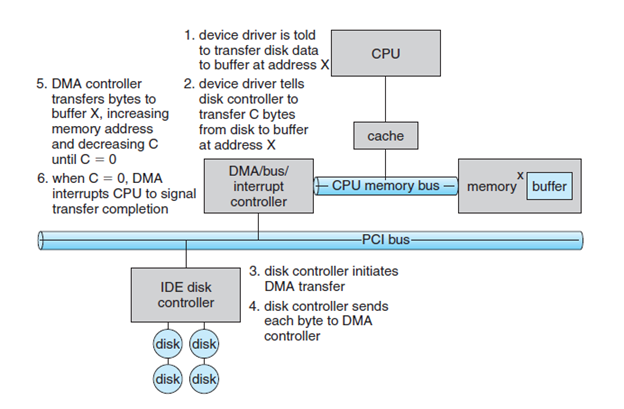
\includegraphics[scale=0.8]{os2.png}
    \caption{Operation of DMA}
    \label{fig:my_label_2}
\end{figure}

\subsection{Steps of DMA transfer}
    \begin{enumerate}
        \item Device driver asks the I/O device to transfer $C$ bytes of data to memory. 
        
        \item I/O device sends DMA request (DRQ) to the DMA controller. 
        
        \item DMA controller accepts the DRQ and asks the CPU to hold (stall) for a few cycles (HLD). CPU acknowledges this and sends and Hold Acknowledgement (HLDA) in response. 
        
        \item DMA controller acknowledges I/O device (DACK) that the data transfer can be performed. 
        
        \item DMA reads one byte at a time and uses the memory bus to write to memory, increasing the memory address and decreasing $C$. 
        
        \item When $C$ is 0, meaning all data is now transferred to memory, DMA sends an interrupt to the CPU signalling end of transfer. 
    \end{enumerate}
\subsection{DMA Operation Modes}
\begin{itemize}
    \item \textbf{Burst Mode}: DMA operates in one burst and releases the memory bus only after the transfer is entirely complete. 
    
    \item \textbf{Cycle Stealing Mode}: In this mode, the DMA controller forces the CPU to stop its operation and relinquish the control over the bus for a short term to DMA controller. After the transfer of every byte, the DMA controller releases the bus and then again requests for the system bus. In this way, the DMA controller steals the clock cycle for transferring every byte.
    
    \item \textbf{Transparent Mode}: Here, the DMA controller takes the charge of system bus only if the processor does not require the system bus.
\end{itemize}

\section{Transforming I/O Requests to Hardware Operations}
\begin{itemize}
    \item The association between a file name and a physical device that the file resides on is OS dependent. 
    
    \item In Windows and DOS, the device name is itself a part of each and every file name (eg: in the filename \texttt{C:\textbackslash Users \textbackslash Desktop \textbackslash a.txt}, the device name is \texttt{C:}, and it is mapped to a device port number using the device table).
    
    \item In UNIX, the \textbf{mount table} associates prefixes in file paths to a specific device. The device name returned by the mount table is looked up in the file system directory, and the returned values are the \texttt{major, minor}. 
    
    \item The major device number identifies a device driver that should be called to handle I/O to this device. The minor device number is used by the driver to access the device table, to return the address (memory mapped or port address) of the device. 
    
    \item The steps in a blocking read() call are:
    
    \begin{itemize}
        \item Read call to the descriptor of a file that has been opened previously.
        
        \item In case of input, if the data is available in the buffer then it is returned to the process and the I/O request is completed. 
        
        \item Else an I/O must be performed. The process is removed from the ready queue and put on the wait queue for the device. Once the process is ready the I/O subsystem sends an I/O request to the device driver. 
        
        \item The device driver creates kernel memory space, and schedules the I/O. Eventually the device driver issues a command to the device controller by writing to the control registers. 
        
        \item The device controller operates the device hardware to perform the I/O. 
        
        \item The DMA setup manages the data transfer. Once the transfer is complete, it sends an interrupt to the CPU. 
        
        \item The correct interrupt handler handles the interrupt, signals the device driver and returns from the interrupt. 
        
        \item The device driver receives this signal, checks to see which I/O request has completed and notifies the kernel I/O subsystem of the completion of that request. 
        
        \item The kernel transfers data or return codes to the address space of the requesting process and moves the process from the wait queue back to the ready queue
        
        \item The process is now unblocked, and once it gets access to the CPU it resumes execution. 
    \end{itemize}
\end{itemize}

\section{Protection}
\subsection{Goals of Protection}
\begin{itemize}
    \item To ensure that intentional access violations do not cause harm to the functioning of the system. 
    
    \item Provide a means to distinguish between authorized and unauthorized usage. This is done by detecting hidden errors at the interfaces between components of the OS, which can lead to contamination by a malfunctioning component. 
    
    \item Provide a mechanism that ensures that policies that govern resource usage are enforced, and allow for flexibility in policy creation (either in the system design, or by the management of the system, or by individual users for their own files).
    
    \item These policies are implemented both by the OS and the application programs, to guard the resources that are used by the application programs.
    
    \item Separation of policy and mechanism allows for multiple policies to be implemented flexibly.
\end{itemize}

\subsection{Principles of Protection}
\begin{itemize}
    \item One of the principles that guides protection system design is the \textbf{principle of least privilege} (ie. users/programs/systems are to be given the bare minimum of privilege that is needed for them to perform their tasks). 
    
    \item Some methods of implementation of this principle are:
    \begin{enumerate}
        \item System calls with fine grained access controls.
        
        \item Mechanisms to enable and disable privileges for a user/system/program as needed.
        
        \item Audit trails for system admins to take stock of all protection related activites on the system.
        
        \item Separate user accounts with privileges only based on the role of that user (Role Based Access Control or RBAC). 
        
        \item Access Control Lists that enable access to specific subsystems (disk/network/remote access) at specific times for each user. 
    \end{enumerate}
\end{itemize}

\subsection{Domain of Protection}
\begin{itemize}
    \item A computer is a collection of processes and objects. Objects may be hardware or software resources. 
    
    \item Each object has a name and some operations that are specific to it. A process should access only those objects that it is authorized to access, and it requires for completion of the task (called the \textbf{need to know principle}). 
    
    \item Every process belongs to one protection domain. The domain is a list of pairs of the form $\langle O_i,  \{ p_1, p_2, p_3 \} \rangle$ where $O_i$ is an object and $p_1, p_2, ...$ are permissions for various operations on that object. 
    
    \item Domains may overlap, ie: they can share access rights for one particular object. 
    
    \item Domains are associated to process either statically (once assigned cannot be changed) or dynamically (process can move between domains). If this association is static, then a mechanism must be there to change the content of a domain 
    
    \item eg: An object $O_1$, process $P_1$ needs read access to $O_1$ in one phase and write access to it in the next. The domain in which $P_1$ is running cannot have both read and write at all times as per the principle of least privilege). 
    
    \item In case of dynamic association between process and domain, a mechanism for domain creation and domain switching is used for the above. 
    
    \item Each user may be a domain, each process may be a domain, or each procedure is a domain. 
\end{itemize}

\subsubsection{Domains in UNIX}
\begin{itemize}
    \item In UNIX users are domains. Each file has an \textbf{userID} and a \textbf{setuid} bit. 
    
    \item If the setuid bit is 1, then any user can execute the file as if they were the owner of the file, meaning that the userID of the file is set to the owner's name.
    
    \item If the setuid bit is 0, then the user runs that file as if they are themselves. There is no change in the userID of the file in this case. 
    
    \item On system programs that should be accessed by all users (eg: networking tools), the setuid is set to 1 and the userID for all is set to \textbf{root}. 
    
    \item In order to enforce protection, the privileged programs may be placed in a single directory owned by root. This prevents intruders from hiding privileged programs with setuid 1 in random locations for later use. 
    
    \item Another protection technique is to prevent userID from changing on the fly. All privileged access must happen via a single \textbf{daemon process} that itself has root as its userID. 
\end{itemize}

\subsubsection{Domains in MULTICS}
\begin{itemize}
    \item Here domains are organized hierarchically into concentric rings. The rings are organized such that ring $D_0$ has the highest privilege and $D_1 < D_0$, $D_2 < D_1$ and so on (ie. inner rings have higher privilege than outer rings). 
    
    \item Each segment of the MULTICS address space is attached to one ring. The segment description includes:
    \begin{enumerate}
        \item Ring number
        
        \item Bits for read/write/execute privileges
        
        \item Access bracket $(b_1, b_2)$ such that $b_1 < b_2$
        
        \item A limit $b_3$ such that $b_3 > b_2$
        
        \item List of gates or access points at which segments can be called. 
    \end{enumerate}
    
    \item A process executing in ring $i$ and calls a segment/procedure with bracket $b_1, b_2$ such that $b_1 \le i \le b_2$ then the call is allowed. Otherwise a trap occurs and the handling is as follows:
    \begin{itemize}
        \item If $i < b_1$, then the call is allowed. However parameters that are passed to a lower priority ring must be copied first. 
        
        \item If $i > b_2$, then the call is allowed only if $i \le b_3$ and the call is directed to one of the entry points in the list of gates. 
    \end{itemize}
    \item The ring structure does not enforce the need-to-know principle. If a process is to be accessible in $D_i$ but not in $D_j$, then $i < j$. But this means that segments in $D_i$ can access segments in $D_j$. 
\end{itemize}

\section{Access Matrix}
\begin{itemize}
    \item The general model of protection involves a matrix where rows are domains and columns are objects. This is called the access matrix. 
    
    \item Each element of the matrix is a set of operations that the domain $i$ can perform on object $j$. 
    
    \item The access matrix also includes columns for domains. The entry $A(D_i, D_j)$ is whether a process in domain $i$ is allowed to switch to domain $j$. 
    
    \item If one of the operations in the entry $A(D_i, O_j)$ has \textbf{copy privilege} (marked as *), then it can copy that operation to any of the other domains only for the resource $O_j$. 
    
    \item Either the copy can be implemented as a propagate (ie. copy to new domain then remove from original), or it can be a single limit copy (ie. the new domain gets a non-copiable right).
    
    \item If $A(D_i, O_j)$ has an \textbf{owner privilege}, then it can add or remove any access right of any domain in that resource $O_j$. 
    
    \item If $A(D_i, D_j)$ has a \textbf{control privilege}, then $D_i$ can remove any access right from the entire row of $D_j$.
\end{itemize}

\subsection{Access Matrix Implementation}
\subsubsection{Global Table}
\begin{itemize}
    \item A table of ordered tuples of the form $\langle$Domain, Object, Access rights list$\rangle$. 
    
    \item The large size of table means it cannot be stored in memory, which means additional I/O cost. Also it does not take care of shared privileges among domains. (eg: if all domains are allowed to read a file, each domain still has to have a separate entry in the table)
\end{itemize}

\subsubsection{Access List for Objects}
\begin{itemize}
    \item Each object has an access list with tuples of the form $\langle$Domain, Access rights list $\rangle$. 
    
    \item This design also allows a default set of operations apart from the list that is defined as part of the domain. This default set is checked if the tuple $D_i, R_i$ does not contain the requested operation. 
\end{itemize}

\subsubsection{Capability List}
\begin{itemize}
    \item Each domain has a list of tuples of the form $\langle$Object, Access right list$\rangle$. 
    
    \item A process executing in a domain requests for the operation by sending the object name (aka the capability). If that capability is possessed then operation is allowed.
    
    \item The capability is not accessible in the address space of all processes working in a domain. It lies in a separate protected memory, that is created by the OS. 
    
    \item Protection for the capability list is enforced using:
    \begin{itemize}
        \item A \textbf{tag} that identifies a capability list as against normal data. Hardware or firmware protection is used to ensure that no process can modify the tag bits. Multiple tag bits allow the OS to further identify other types of data as well. 
        
        \item Memory is segmented into a space for data and another space for capability list that can only be accessed by the OS. Segmentation of memory implements this easily. 
    \end{itemize}
\end{itemize}

\subsubsection{Lock and Key Mechanism}
\begin{itemize}
    \item Each object has a list of unique bit patterns called locks.
    
    \item Each domain has another list of bit patterns called keys.
    
    \item  A process executing in a domain is allowed to access an object only if the domain has one key that matches one of the object's locks 
    
    \item Similar to capability lists, the memory where these locks and keys are stored must be protected from the user and only accessible/manageable by the OS. 
\end{itemize}

\subsubsection{Comparison of all the above}
\begin{itemize}
    \item Global table is simple to implement but space inefficient.
    
    \item Access List for object is logical from user point of view, but modifying privileges for a single domain is complicated, and searching in long access lists (as is done for each object access) is time consuming. 
    
    \item Capability lists are efficient from a process point of view, but revocation of capabilities is inefficient. 
    
    \item Lock and Key is a compromise between access list and capability list. The keys can be passed freely from domain to domain. In addition, access privileges can be effectively revoked by the simple technique of changing some of the locks associated with the object. 
\end{itemize}

\section{Access Control and Revocation of Access Rights}
\begin{itemize}
    \item Solaris 10 implements \textbf{Role Based Access Control} (RBAC). 
    
    \item A privilege is the right to use the system call or a specific option in a system call (eg: write option in file open() call). 
    
    \item Privileges can be assigned to processes. 
    
    \item Privileges can also be assigned to \textbf{roles}, and roles can be assigned to users. 
\end{itemize}

\subsection{Revocation}
\begin{itemize}
    \item Immediate vs delayed. If delayed, when will revocation take place?
    
    \item Selective vs general. If an access right for an object is revoked, does it affect all users who have an access right to that object, or can a subset of users be specified?
    
    \item Partial vs total. Can only a subset of rights be revoked for an object, or must all the rights be revoked for it?
    
    \item Permanent vs temporary revocation. 
    
    \item Features to be implemented by all revocation systems are:
    \begin{itemize}
        \item \textbf{Reacquisition}: If a capability has been removed from a domain (as is done periodically), a process running in the domain must be allowed to reacquire it unless it has been revoked. 
        
        \item \textbf{Back-Pointers}: Each object maintains a list of pointers pointing to capabilities of that object. If revocation is needed, then the pointers can be followed to modify the capabilities as necessary. This is general but costly. 
        
        \item \textbf{Indirection}: A capability points to an entry in a global table that points to an object. Revocation is done by deleting that table entry. Now the capability, if accessed, points to an invalid table entry. This does not allow selective revocation for a subset of users. 
        
        \item \textbf{Keys}:
        \begin{enumerate}
            \item Each object has a master key. When a capability is created, its key is associated with the master key of the object. 
            
            \item Revocation is changing the master keys, hence all the capabilities with the object are revoked. 
            
            \item This does not allow for selective revocation, unless each object has several master keys. These master keys are grouped into one table, and revocation means removing that key from that global table. 
            
            \item One key can associate with many objects, and many master keys can associate with one object. This allows for flexibility. 
            
            \item A policy decision is the privilege of editing keys (create, update, delete). Whether the owner of the object should be allowed to do these is up to the designer to implement. 
        \end{enumerate}
    \end{itemize}
\end{itemize}

\section{Security}
Secure system is one that only allows resources to be used legally and in the intended manner, under all circumstances irrespective of the malicious (or otherwise) intent of the user. 

\subsection{Types of Security Violations}
\begin{itemize}
    \item \textbf{Breach of Confidentiality}: Unauthorized reading of data
    
    \item \textbf{Breach of Integrity}: Unauthorized modification of data
    
    \item \textbf{Breach of Availability}: Unauthorized destruction of data (eg: website defacement)
    
    \item \textbf{Theft of Service}: Unauthorized use of resources
    
    \item \textbf{Denial of Service}: Preventing legitimate use of the system by authorized users. 
\end{itemize} 

\subsection{Types of Security Attacks}
\begin{itemize}
    \item \textbf{Masquerading}: Impersonating a legal user to gain access to a sensitive communication. This is done by \textit{breaching authentication}. 
    
    \item \textbf{Replay Attack}: Repeat of a legal communication in order to illegally get access to resources. It can be done as an exact replica, or can be done with \textit{message modification} to extract further higher privileges. 
    
    \item \textbf{Man-in-the-middle Attack}: A third party intercepts the current ongoing communication session using \textbf{session hijacking}, and poses as the sender to the receiver, thus listening to all information exchanged. 
    
    \item \textbf{Phishing}: A portal that tricks legitimate users into giving up confidential information without their conscious knowledge of it being used for malicious purposes. 
\end{itemize}

\subsection{Levels of Security}
\begin{itemize}
    \item \textbf{Physical}: Physical security against human intruders. 
    
    \item \textbf{Human}: Careful user authentication
    
    \item \textbf{OS}: Protection of system from revealing sensitive information and harming the capabilites of the system (eg: buffer overflow, runaway processes causing DOS attack)
    
    \item \textbf{Network}: Intercepting sensitive information travelling over networks. 
\end{itemize}

\section{Program Threats}
\subsection{Trojan Horse}
\begin{itemize}
    \item A code segment that misuses it's environment is called a Trojan Horse. 
    
    \item Many systems have mechanisms for allowing programs written by users to be executed by other users. 

    \item If these programs are executed in a domain that provides the access rights of the executing user, the other users may misuse these rights.
    
    \item \textbf{Spyware} is a variation of Trojan horse software wherein such software comes bundled with user applications. 
    
    \item The role of spyware is to display ads, or open pop up windows or capture information from the user's system and send it back to a central site. 
    
    \item Such attacks are generally classified as \textbf{covert channel} attacks. 
\end{itemize}

\subsection{Trap Door}
\begin{itemize}
    \item An intentional security breach left behind by the developer of the program. 
    
    \item Example: A banking application that rounds up and sends the extra fraction of money to the programmer's account. 
    
    \item Compilers can generate trap doors along with object code for the given source code. As these trap doors cannot be located in the file system this is a more nefarious attack. 
\end{itemize}

\subsection{Logic Bomb}
\begin{itemize}
    \item A program that initiates a security breach in the system only under specific conditions of operation is called a \textbf{logic bomb}. 
\end{itemize}

\subsection{Stack and Buffer Overflows}
\begin{itemize}
    \item The sequence of steps in a buffer overflow attack are:
    \begin{enumerate}
        \item Overflow an input field (command line argument or STDIN), on a network daemon for example, until it writes into the stack. 
        
        \item Overwrite the current return address on the stack with the address of the code that is loaded in step 3. 
        
        \item Write a code that performs malicious activities on the system (eg: start a shell process). 
    \end{enumerate}
    
    \item The goal is to overflow the return address field in the stack frame that contains the address that the function returns control to once it finishes executing. 
\end{itemize}

\subsection{Viruses}
\begin{itemize}
    \item A virus is a self-replicating fragment of code embedded in a legitimate program, that is used to "infect" a computer system. 
    
    \item \textbf{Virus Dropper} is a software that inserts a virus into a system. It is commonly implemented in the form of a \textit{Trojan Horse}.
    
    \item Categorization of Viruses:
    \begin{itemize}
        \item \textbf{File Virus}: A standard file virus infects a system by appending itself to a file. It changes the start of the program so that execution jumps to its code. After it executes, it returns control to the program. 
        
        \item \textbf{Boot Sector Virus}: Loads at every boot time, infects other devices that are also loaded at boot time. 
        
        \item \textbf{Macro Virus}: Virus written in a high-level language that runs along with high-level user applications. 
        
        \item \textbf{Source-Code Virus}: A source code virus looks for source code and modifies it to include the virus and to help spread the virus.
        
        \item \textbf{Polymorphic}: One that changes its form each time it is installed, in order to avoid detection by anitvirus software. This is done by changing not the functionality but the signature of the virus. 
        
        \item \textbf{Encrypted Virus}: In order to avoid detection, the virus is installed in encrypted form and decrypted (with another installed decryption code) before execution. 
        
        \item \textbf{Stealth Virus}: Attempts to avoid detection by modifying parts of the system that could be used to detect it. For example, it could modify the read system call so that if the file it has modified is read, the original form of the code is returned rather than the infected code
    \end{itemize}
\end{itemize}

\section{System and Network Threats}
\begin{itemize}
    \item OSes strive to reduce their \textbf{attack surface}s (possible exploitable vulnerabilities).
    
    \item This is mainly done by reducing openness, ie. number of available services and functionalities. 
\end{itemize}

\subsection{Worm}
\begin{itemize}
    \item A worm consists of a \textbf{grappling hook} (aka vector) program and a main program. 
    
    \item The job of the grappling hook is to connect to the original system where it was uploaded, and copy the main program to that machine. It effectively spreads the main program to as many targets as possible. 
    
    \item Morris' worm is one popular example of a worm program (written in 1998, used to infect computers on the internet). 
    
    \item The grappling hook programs were propagated using three main tools: the \textbf{rsh} tool, the \textbf{finger} tool and the \textbf{sendmail} tool.
    
\end{itemize}

\subsubsection{RSH attack}
\begin{itemize}
    \item \textbf{rsh} is an UNIX utility for remot shell access. 
    
    \item \textbf{rsh} allows users not have to repeatedly enter passwords for networks by maintaining a file with host and username pairs. The worm searched these files for sites that could be accessed without passwords and opened remote shells on those machines. 
    
    \item Once rsh was used to establish remote shell access, the main worm could be run. 

\end{itemize}

\subsubsection{Finger attack}
\begin{itemize}
    \item The \textbf{finger} tool gives information about a specific host on the internet (like username, real name, phone no. etc). 
    
    \item The worm executed a buffer-overflow attack on finger by sending it a a 536-byte string crafted to overflow the buffer. 
    
    \item Instead of returning to the main routine where it resided before the worm's call, the finger daemon was routed to a procedure within the invading 536-byte string now residing on the stack.
    
    \item The new procedure executed \texttt{/bin/sh}, which, if successful, gave the worm a remote shell on the machine under attack.
\end{itemize}

\subsubsection{Sendmail attack}
\begin{itemize}
    \item Sendmail is an SMTP client that routes and stores e-mails. 
    
    \item Debugging code in the utility permits testers to verify and display the state of the mail system.
    
    \item Morris included in his attack arsenal a call to debug that issued a set of commands that mailed and executed a copy of the grappling-hook program.
\end{itemize}

\begin{itemize}
    \item As the worm spread to a new system, it checked the system for a copy of itself. If found, the worm would exit, except in every 7th instance. 
    
    \item This was done as a means to avoid baiting with fake copies of the worm program. 

\end{itemize}

\subsection{Port Scanning}
\begin{itemize}
    \item Not an attack methodology, but a way of scanning ports and seeing the services run on them. 
    
    \item An attacker can run a port scanner, detect any vulnerable software running on any port and target that service specifically. 
    
    \item Utilities such as \textbf{nmap} are used for this purpose. When pointed at a target, it will determine what services are running, including application names and versions, the host operating system, and information about defenses, such as what firewalls are defending the target. 
\end{itemize}

\end{document}